\hypertarget{status-report}{%
\section{Status report}\label{status-report}}

Task~\taskref{component-architecture}{workflow} of
\WPref{component-architecture} aims to improve the development workflow in
mathematical software, to ease contributions by all actors, from experts
developers on those projects or coming from other projects, to students, novice
users, or non-programmers.

For this deliverable we focused on engaging newcomers to become contributors by
reducing the barrier of entry to \Sage development. In particular, trivial
contributions ought to be trivial: for example, a user or technical writer that
notices a typo or a potential phrasing improvement in the documentation should
be encouraged and empowered to fix it on the spot and submit it for review and
integration into \Sage.

The Sage community has a history of blurring the line between developer and
user, with even new users often encouraged to make code contributions.
However, the core group of frequent development contributors remains relatively
small, and has a well-established workflow and culture surrounding its existing
development tools--in particular the source code hosting and issue tracking
service \Trac.  This works well for experienced Sage developers, but also
creates certain barriers to entry for new contributors, especially those who
are new to open source development.  Therefore we sought solutions to better
integrate Sage's Trac-based workflow with platforms that are more modern and
familiar to open source novices, such as \GitHub and \GitLab, without
immediately breaking the Sage project's existing workflow.\footnote{Upon
writing the proposal we envisioned using \SMC (now \cocalc) as a major
development platform for Sage, hence the title of this deliverable.  However,
while \cocalc remains quite viable for this purpose, it became evident that
there was a need for solutions not explicitly tied to \cocalc.  See Section
\ref{redesigned-work-plan} for discussion.}

Nevertheless, we believe that this will also open the doors to long-term
improvements in Sage's development workflow, as the advantages of using these
new tools become more apparent.  Part of this work also serves as a
prerequisite to improvements in Sage's continuous integration practices, which
are being explored in
\longdelivref{component-architecture}{multiplatform-buildbot}.

An aspect that Sage (and indeed any open source mathematics software) prides
itself on over closed-source alternatives is the ability to peer inside the
software to see how it works.  It is not a black box and one does not have to
take its results for granted--it is possible to look at the source code in
order to understand how a particular algorithm works, or even modify and
improve it.  To this end we sought ways to more tightly couple Sage's API
documentation to its source code--and through access to the source code,
encourage contribution of improvements.

To these ends, this deliverable includes the following improvements to Sage's
development platform and documentation:
\begin{enumerate}
\item Enable users with existing GitHub credentials to log into Sage's
    Trac site.
\item Create a presence for Sage on the GitLab collaborative source code
    sharing service, including the ability to accept patches to Sage's
    documentation and source code in the form of {\em merge requests}
    (a.k.a.~{\em pull requests}).
\item Link \GitLab merge requests to tickets in Sage's Trac issue tracker in
    a manner that fully integrates with Sage's existing development workflow.
\item Create a direct path from Sage's online API documentation to the source
    code, and from the source code directly an interface to edit the source
    code and submit a patch (as a merge request) all without the user having to
    leave their web browser.
\end{enumerate}


\hypertarget{redesigned-work-plan}{%
\section{Redesigned work plan to best achieve the deliverable aim\label{redesigned-work-plan}}}

This deliverable was originally entitled "Integration between SageMathCloud and
Sage's TRAC server". The vision and rationale were as follows: Compiling Sage
and its dependencies requires a significant amount of computing power, and also
a number of development software prerequisites that can be hard to set up on a
developer's personal computer, especially in the context of a one or two day
workshop.

At the time of the proposal, \cocalc (then still named \SMC) had recently begun
providing a cloud-hosted virtual environment that was immediately suited to
building, running, and developing Sage. This looked promising and we envisioned
that users doing development on Sage in a \cocalc environment ought to have a
way to submit their development efforts directly to Sage's \Trac (hereafter
referred to as Sage-Trac).

We started the work on this deliverable by an in depth review of its aim--
reducing the entry barrier to Sage-development--and best means to achieve it.

We noted that the existing command-line development tools for Sage (e.g.~the
community-maintained {\tt git trac} utility) already provided integration with
\Trac independently of the development environment, and had gained wide
adoption by the community. So it was unclear exactly what the advantage would
have been to adding features to \cocalc solely for the purpose of integrating
with Sage-Trac, especially since those features would be very specific to Sage
and would not integrate well into the direction \cocalc has moved in, as a more
general-purpose computing environment.  It was also unclear how many people
were actually using \cocalc as their primary platform for Sage development,
while it is certain that most of the core Sage developers are not doing so.

Additionally, as previously noted, modern cloud-based code sharing and issue
tracking sites such as \GitHub and \GitLab have been gaining incredible
momentum, and almost anyone working on modern open source projects--be they
veteran developers or novices--are likely to have encountered them and be
familiar with them.  They are also backed by large companies and sponsors and
are unlikely to go away soon.

Meanwhile \Trac, while an excellent system and familiar to many developers who
worked with it in the early 2000's, is showing its age.  The \Trac software has
few active developers anymore, and relative difficulty of setting up a
self-hosted Trac-based project (as opposed to the near zero effort of adding a
project to cloud-based services) means very few new projects are adopting it.

Therefore it seemed a better focus of our efforts to open Sage's development
workflow up to the use of more modern development platforms (see the next
section for discussion of how we are integrating \GitLab into the workflow).
We expect this will have benefits in the future--more modern development tools
integrate well with services like \GitHub or \GitLab out-of-the-box, whereas
integrating development tools \Trac requires extra work on the part of the Sage
community that might be better spent elsewhere.

Finally, we have had some discussion about how to integrate issue tracking and
source code contributions into VREs in general (not just \cocalc), and while no
consensus has emerged as to what form this would take (Would one submit issues
against a VRE? Against the libraries and software it uses?  Both?), it would
most likely integrate best with modern code-sharing services.


\hypertarget{description-of-the-achievements}{%
\section{Description of the
achievements}\label{description-of-the-achievements}}

\hypertarget{trac-github-login}{%
\subsection{Login to Trac via GitHub usernames}\label{trac-github-login}}
A perennial problem in managing the Sage community's self-hosted \Trac site has
been dealing with user registration and authentication.  As with many
bug-tracking sites, Sage-Trac requires users to register and log into the site
in order to post bugs and feature requests.

Allowing anyone on the internet to register an account--not to mention allowing
anonymous users to post to the site--regularly opened it up to a flood of spam.
Even adding CAPTCHAs to the registration process was not fool-proof, as
CAPTCHAs are being defeated more and more by either machine learning or cheap
manual labor.  Therefore, for several years the Sage community has resorted
to a process of manual user registration: potential users of the site would
send an e-mail to a dedicated address with a manually written application form,
and eventually a site administrator--if the application appeared genuine--would
approve the application and assign the user a username and temporary password,
again over e-mail.

This process has worked, and does not generally leave anybody out.  But it is
still a slow, and labor-intensive process.  One would not be surprised if it
has discouraged potential bug-reports, with users deciding it was not worth
their time, or forgetting about the issue while waiting for their account
registration to be approved.

Therefore, we sought to make logging into Sage-Trac a more painless and
instantaneous process.

\GitHub, with its over 40 million users as of writing, is the largest source
code hosting site in the world.  Many people, even who are not full-time
software developers, have a GitHub account if they have worked at all
peripherally with open source software (if nothing else, in order to submit bug
reports to projects).  By making it possible to log into Sage-Trac with one's
existing GitHub account, this opens Sage development up instantly to any of
those 40+ million users without additional effort.  To date, this has not
contributed any spam to Sage-Trac either, as we are able to leverage GitHub's
own spam management.

We still also allow existing accounts to log in, and maintain the manual
registration system so that users who do not already have, or prefer not to
obtain GitHub accounts may be registered.  However, in the four months since
launching this new feature on February 27, 2018, nearly one fourth (31 out of
130) of the users who submitted new tickets were logged into the site using
GitHub.  Of the other 130, only a handful were new manual registrations, while
the rest were using accounts they already had on the system before February 27.
We expect the number of contributions from GitHub users to grow, and will
consider adding the ability to log in via other external authentication
providers, such as \GitLab and Google.


\hypertarget{gitlab-trac-integration}{%
\subsection{\GitLab-\Trac integration}\label{gitlab-trac-integration}}

While making it easier for new contributors to \Sage to log into its \Trac site
eliminates one barrier to contribution, another barrier is learning its
somewhat unique development and source code contribution and review workflow.
This workflow is well-documented and custom tooling is provided to make it
easier (e.g.~the {\tt git trac} command for posting Git branches directly to
Trac from the command line); nevertheless it is still not an entirely familiar
workflow for anyone new to Sage--experienced developers and novices alike.
%
Experience gained through our many training workshops suggests that it usually
takes a one hour demo and a couple walk-me-through first contributions (often
spread over several such workshops) to get used to the workflow and become
autonomous. And few people--mostly already advanced programmers--learn the
workflow by themselves outside of training workshops, even for trivial
contributions.

Novices in particular--especially those who became involved in open source
development within the last five years--will tend to be more familiar with what
is known as the "GitHub
Workflow"\footnote{\url{https://guides.github.com/introduction/flow/}} as was
popularized by \GitHub.\footnote{Sage's existing process is not that different
from the GitHub workflow, but small differences in semantics and user
experience make this less immediately obvious.} Thus, the availability of a
complementary GitHub-like workflow would lower the barrier to contributions.
As we will see in the next section, this also makes it easier to go directly
from browsing Sage's documentation to making small source code and
documentation contributions.

In order to accomplish this, we might have used a mirror of Sage's Git
repository on \GitHub (indeed, such a mirror already exists).  However, for
this purpose we chose instead to focus on \GitLab--a competitor to \GitHub that
provides a similar product, but with an {\em open core} business model, meaning
that the majority of the software that runs the service \url{GitLab.com} is
provided under an open source license, while the company maintains optional
"enterprise" features under a separate proprietary license.  A few reasons we
chose \GitLab for this purpose over \GitHub include:

\begin{enumerate}
\item Many members of Sage's community have strongly-held political objections
    to relying on closed-source commercial software for development, and would
    be reluctant to adopt GitHub into their workflow (the aforementioned GitHub
    login for Trac being acceptable due only to it being optional).  We hope
    that GitLab, itself being {\em mostly} open source, will be a more
    politically viable alternative. Sage itself being an open source project,
    we are happy to work hand-in-hand with other open source projects.

  \item Although we now host a mirror of the Sage project on
    the cloud-based \url{GitLab.com} {\em service}, should the need
    arise for any reason we could easily migrate this mirror to a
    any other instance of the GitLab service, e.g. self hosted using
    GitLab's {\em software}.

    Indeed, the Sage community has long prided itself on being almost entirely
    independent of commercial products or services for hosting its
    development tools; while using \url{GitLab.com} is convenient (less
    effort spent on server maintenance that could be spent improving Sage
    itself), it is encouraging to know that the possibility exists.

\item \url{GitLab.com} allows users to log in with their GitHub usernames, Google
    accounts, and other third-party authentication providers (in addition to
    registration directly with GitLab).  Thus, although GitHub has a wider
    existing user base, all users with GitHub accounts can log into GitLab
    without significant effort.

\item GitLab has some features that are not present on GitHub.  In particular,
    GitLab has a powerful built-in continuous integration and deployment
    platform that we have found well-suited for Sage.  Our efforts in using
    GitLab's continuous integration/deployment tools are reported on in
    \longdelivref{component-architecture}{multiplatform-buildbot}.  Some of
    this work directly impacts
    Task~\taskref{component-architecture}{workflow} by reducing the entry
    barrier to the {\em review} part of the development workflow.

\item Although GitLab the company is currently based out of San Francisco
    (albeit with only one employee at its San Francisco office) the project
    was started in Europe (Ukraine) and a large portion of its all-remote
    employees are based in Europe.
\end{enumerate}

For these reasons, among others, we have set up a new
mirror{\footnote{\url{https://gitlab.com/sagemath/sage}} of Sage's Git
repository on GitLab, with the ability to accept contributions in the form of
{\em merge requests}, which are the same as what GitHub calls "pull requests".

\TODO{This note might come a bit late in the text; it could possibly
  be a footnote earlier on. Or not.}
Note: The choice of GitLab for hosting a Sage project may appear to stand in
contrast with the previous section of this deliverable, which added
authentication to Sage-Trac via {\em GitHub}.  However, as noted above, GitLab
also allows authentication with GitHub accounts, taking advantage of GitHub's
existing wide user base.  Therefore, we focused primarily on GitHub-based
authentication.  In the future we would also like to add the ability for users
to authenticate with Sage-Trac via GitLab, if there is demand for it.

The challenge in opening up Sage to accepting contributions via GitLab was
doing so in a way that did not significantly disrupt Sage's existing Trac-based
development workflow and to make gradual introduction of a new kind of workflow
more socially acceptable; the community indeed tends to have strong opinions on
the subject.

Our solution was to implement a plug-in for Sage-Trac that uses GitLab's API to
automatically open a {\em ticket} on Sage-Trac for each merge request opened on
GitLab.  That way, Sage developers watching Sage-Trac for new contributions are
notified even without having to go to GitLab.  The proposed code changes in the
merge request--which are hosted on GitLab--are also automatically synchronized
to Sage's main Git repository, so that all of Sage's existing maintenance tools
continue to work as normal even for contributions that came originally through
GitLab.  When a ticket is {\em closed} on Sage-Trac (i.e.~the changes were
accepted, or rejected) the corresponding merge request on GitLab is also
automatically closed.  In this way, veteran Sage developers may, if they wish,
accept contributions through GitLab without ever actually having to go to
GitLab.

That said, we hope that most of the Sage development community {\em will}
consider using GitLab.  In particular, we believe that the more modern code
review tools provided by GitLab will prove too compelling to ignore.  There
is a small risk associated with this: many code change tickets generate
discussion--sometimes a significant amount--in the form of code review comments
or sometimes even debate.  If an issue is tracked on both Sage-Trac and on
GitLab, there is a risk of that discussion becoming fragmented between the two
sites and difficult to follow.  This can be mitigated either through policy
(e.g.~keep discussion of a single issue on one site or the other, but not
both), or in the form of a technical solution (e.g.~enhance the existing
synchronization plug-in to synchronize discussions between the two sites; this
is non-trivial, however).

\TODO{it could be nice to mention that the author of this report is
  also a Trac developer, which highlights that there is no personal
  bias in the point of view expressed here.}

Either way, there is prior art for this process of adopting a modern code
sharing site while maintaining a legacy issue tracking system.  Most notably,
the CPython project (the reference implementation of the Python language and
its standard library--what is typically referred to as just "Python") switched
to a similar model beginning in February 2017: Issues are still tracked
primarily on the project's legacy bug tracking system--which carries in it a
wealth of historical knowledge and lingering open issues--while bug fixes and
new features can be submitted as pull requests on GitHub which are
automatically linked to their corresponding issues on the legacy system.  Since
then, over
6500\footnote{\url{https://github.com/python/cpython/pulls?utf8=\%E2\%9C\%93\&q=is\%3Apr+is\%3Aclosed+is\%3Amerged}}
merge requests have been accepted through GitHub.  In an informal
query\footnote{\url{https://mail.python.org/pipermail/python-dev/2018-February/152200.html}}
to the CPython core developers one year after switching to the new hybrid
workflow, its primary architect, Brett Cannon, asked how the new workflow was
working and the response was overwhelmingly positive.  Frequently cited as a
benefit were the several bots that were created by the community to help manage
pull request submissions.  Many of these bots would be useful for Sage as well,
and although they were created to run on GitHub, the GitLab API is
similar-enough that these bots could be ported to GitLab with minimal effort.
There was also a general interest (including by Python's creator Guido van
Rossum) to move forward with migrating all issues to GitHub, and setting the
legacy bug tracker to read-only; the details of this migration, however, remain
a subject of debate.\footnote{\url{https://lwn.net/Articles/754779/}}  We
believe a similar outcome for Sage's partial migration to GitLab would be
desirable, but it remains to be seen how well it will be adopted by the Sage
community.


\hypertarget{source-in-documentation}{%
\subsection{From Sage API documentation to source code contributions}\label{source-in-documentation}}

As mentioned in the introduction, a selling point of Sage over closed-source
mathematics software is easy access to the source code; the ability to actually
inspect its algorithms--and maybe even improve them--rather than simply plug in
input an trust that the output is correct.

Sage has always made it easy to view the source code for its classes and
functions, not just by downloading and viewing the sources directly, but also
at runtime using its detailed inspection capabilities.  For example, to see the
source code for Sage's {\tt Integer} class it is possible, at the Sage input
prompt, to write {\tt Integer??} (this is in fact a standard feature of the
\IPython interface upon which Sage's user interface is built).

However, the command prompt is not always the easiest place to explore Sage's
capabilities--sometimes reading the online documentation gives a bigger
picture. Reciprocally, while the documentation includes English language prose
and usage examples that explain what different classes and functions do,
sometimes browsing the source code helps get the full picture.

To this end, we have
added\footnote\url{https://trac.sagemath.org/ticket/25914}} two new hyperlinks
that appear in the headings of the API documentation for all classes, methods,
functions, and other documented objects in Sage.

\begin{figure}[!ht]
    \centering
    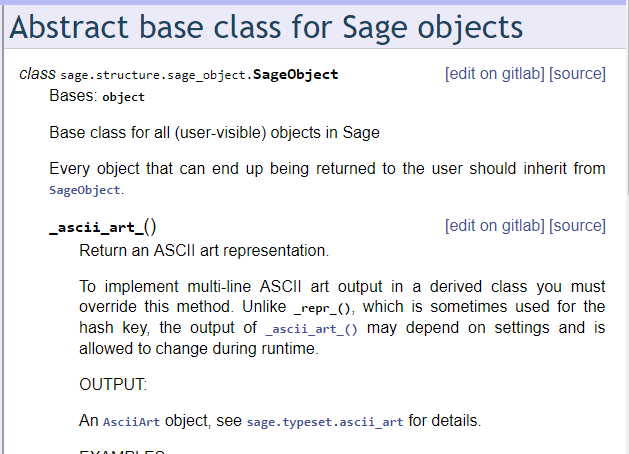
\includegraphics[width=\textwidth]{screenshots/source-links}
    \caption{Example Sage API documentation with new source links.}
    \label{fig:source-links}
\end{figure}

The {\tt [source]} link displays the source code (in this case for the {\tt
EuclideanDomains} class) in the context of the source file it's defined in,
without leaving the Sage documentation site (\url{http://doc.sagemath.org}).
The second link, {\tt [edit on gitlab]}, is what partially motivates having a
mirror of the Sage repository hosted on GitLab, with the ability to accept
merge requests, as described in the previous section.  This feature is inspired
by a similar feature used by the Astropy project in its API
documentation\footnote{See for example \url{http://docs.astropy.org/en/stable/api/astropy.units.Quantity.html\#astropy.units.Quantity}}.

This link opens the source file containing the object in question (e.g.~{\tt
EuclideanDomains}) in the source code browser for the Sage project on GitLab
(see Figure \ref{fig:edit-on-gitlab}).  Users who are logged into, or who
subsequently log into their GitLab accounts, then have the option to edit that
source file directly in the browser using the web-based code editor provided by
GitLab.  Because most users do not have permission to edit the Sage source code
directly, when they save their changes this results in a Git commit to the
user's personal copy of the repository, and a {\em merge request} is opened in
the main Sage repository.  With the GitLab-Trac integration this also results
in a ticket on Sage's Trac for the requested changes to the code and/or
documentation.

\begin{figure}[!ht]
    \centering
    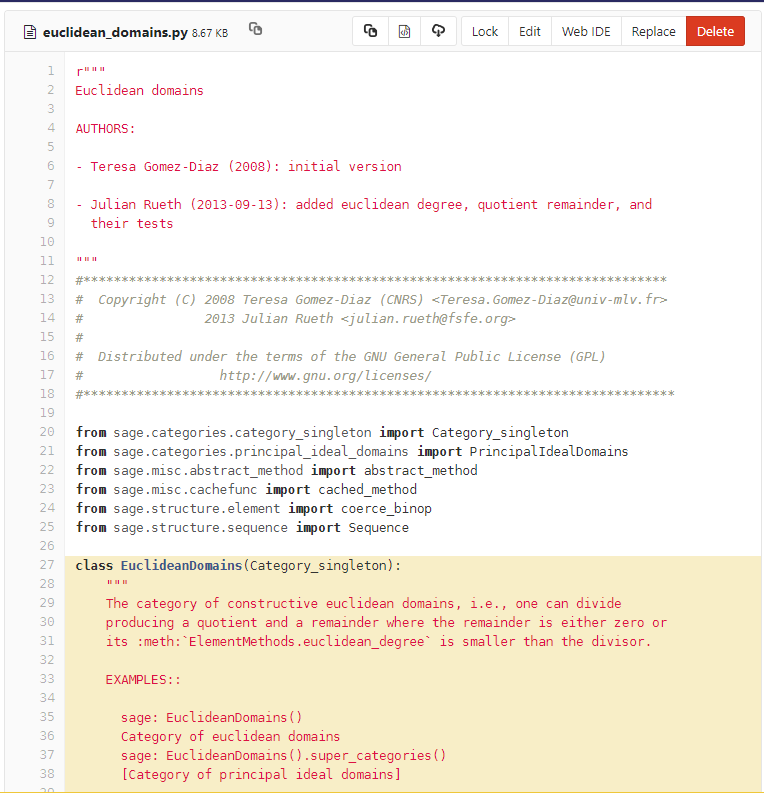
\includegraphics[width=\textwidth]{screenshots/edit-on-gitlab}
    \caption{Editing Sage source code on GitLab via documentation link.}
    \label{fig:edit-on-gitlab}
\end{figure}

In addition to API documentation, much of which is automatically generated from
the source code, Sage also has a large amount of prose documentation in English
and other languages, such as high-level usage documentation for Sage and
tutorials.  This material is all also tracked in Sage's source code repository,
and is something we want to make easy to crowd-edit.  Therefore we also add an
{\tt [edit on gitlab]} link on all the prose documentation, which works the
same as for the API documentation: users are allowed to edit the source files
for the prose documentation and submit their edits as merge requests.  This
would be encouraged for anything from typos and minor clarifications, to
major documentation updates.  By making it a process of a few clicks to from
a reader of the documentation to proposing edits, we believe the will lead
to more rapid quality improvements in Sage's documentation.


\hypertarget{future-work}{%
\section{Future work}\label{future-work}}

\TODO{In the Jupyter notebook (aka VRE) link from Integer? and
  Integer?? to the corresponding help page; maybe direct links to edit
  on gitlab/sources. How far are we from it?}

\TODO{Discuss how this integrates naturally(?) in the VRE?}

\TODO{Once a PR has been created, make it easy for the author to
  browse the generated documentation, from the PR page, ideally
  with a direct link to the relevant doc page. Maybe access
  the binder image too, without having to go through the trac ticket.
}

\TODO{Future steps: simplify non only trivial contributions but also easy one (e.g. involving a code change);
  possibly from a VRE (e.g. a jupyterhub):
  - make sure that the %edit magic works
  - in-place build of the library
  - live reload???
  - anything that could help create a PR/ticket from local modifications?
  - inclusion of git-trac as sagemath package
}


%%% Local Variables:
%%% mode: latex
%%% TeX-master: "report"
%%% End:
